\begin{figure*}[t]
\centering
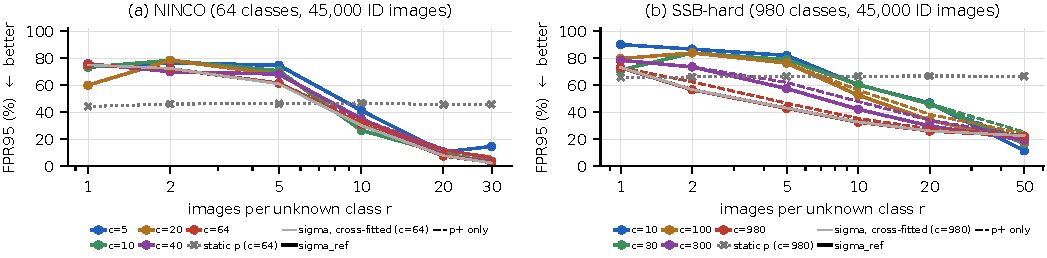
\includegraphics[width=\textwidth]{figs/fig22_rec.pdf}
\caption{再出現と混入率（\FPR{}，単体，DINOv2 L/14 + DINOv3 L/16）．IDの検証画像45,000枚に，NINCO（a）またはSSB-hard（b）から$c$個の未知クラス$\times$$r$枚を加えたテスト集合（クラスと画像の選び方を変えた3回の平均）．実線は$\sR$，破線は$\pP$だけ（参照画像で読む），灰色の点線は静的$p$，灰色の細い実線は交差適合した$\sigma$（後二者は$c$が最大の条件）．}
\label{fig:rec}
\end{figure*}

同じクラスが何枚あり，どの混入率から効くのかを，OpenOODのIDの検証画像45,000枚に，NINCO（64クラス）またはSSB-hard（980クラス，各50枚）から$c$個の未知クラスを$r$枚ずつ加えたテスト集合で実測した（\figref{rec}，全条件は付録\ref{sec:app_rec}）．

\textbf{再出現しない未知には静的な検出器より劣る．}$r\le5$では，$\sR$は同じ特徴の静的$p$より\FPR{}が高く（\NRRecNLeFive{}条件中\NRRecLeFiveWorseStatic{}条件），差の平均は$r{=}1$で\NRRecROneMeanD{}，$r{=}2$で\NRRecRTwoMeanD{}，$r{=}5$で\NRRecRFiveMeanD{}ポイント，最大\NRRecLeFiveMaxD{}ポイントである．NINCOの64クラス$\times$1枚では$\sR$も$\pP$だけも\NRRecNincoCSixtyFourROne\%に対し，静的$p$は\NRRecNincoCSixtyFourROneStatic\%である．1枚だけの未知は$k_g{=}10$本の辺をすべて外へ張るので，伝播はその画像を隣のIDに均す．付録の一つの量$h$は$r\le2$の\NRRecHvsRefLeTwoN{}条件でさらに平均\NRRecHvsRefLeTwoMeanD{}ポイント悪い．$r\ge10$では逆転し（\NRRecNGeTen{}条件中\NRRecGeTenBetterStatic{}条件，差の平均\NRRecGeTenMeanD{}），NINCOの64クラス$\times$10枚で\NRRecNincoCSixtyFourRTen\%，30枚で\NRRecNincoCSixtyFourRThirty\%（静的$p$は\NRRecNincoCSixtyFourRThirtyStatic\%）まで下がる．SSB-hard（兄弟クラス）は遅く，980クラス$\times$10枚で\NRRecSsbCNineEightyRTen\%，50枚で\NRRecSsbCNineEightyRFifty\%である．$\sR$と$\sigma$の差は\NRRecNCells{}条件中\NRRecNWithinOneSig{}条件で1ポイント以内（最大\NRRecMaxAbsDiffSig{}）である．

\textbf{混入率が低いときの種はIDが多い．}混入率1\%未満では，\NRSeedLtOneCellsViews{}のセル$\times$ビューのうち種が選ばれたのは\NRSeedLtOneWithSeeds{}だけで，選ばれたときに種に混じるIDの割合は平均\NRSeedLtOneIdFrac{}（\NRSeedLtOneIdFracMin--\NRSeedLtOneIdFracMax）と水準$q{=}0.2$を超える．種が選ばれない場合を0と数えた偽発見割合（命題3が期待値を抑える量）の平均は\NRSeedLtOneFdpUncond{}，混入率1--10\%で\NRSeedOneToTenFdpUncond{}，10\%以上で\NRSeedGeTenFdpUncond{}で，混入率が高いと水準を超える（較正画像とテスト画像のずれ；\secref{fdp}）．低い混入率でまれに選ばれる種は半分近くがIDであり，種が効くのは同じクラスの未知がそれより多く再出現するときである．

\textbf{分離の上界の実測．}系2の上界は格子の全条件・全未知画像で成り立ち（違反0），上界だけから$\pfin\le0.05$が言える未知の割合は，NINCOの$r{=}30$で\NRBdRefNincoRThirtyCertMin--\NRBdRefNincoRThirtyCertMax\%（実際に$\pfin\le0.05$の割合は\NRBdRefNincoRThirtyActMin--\NRBdRefNincoRThirtyActMax\%），$r\le5$では最大\NRBdRefLeFiveCertMax\%，SSB-hardの$r{=}50$では未知クラスの数とともに\NRBdRefSsbCTenRFiftyCert\%（$c{=}10$）から\NRBdRefSsbCNineEightyRFiftyCert\%（$c{=}980$；実際は\NRBdRefSsbCNineEightyRFiftyAct\%）へ下がる（付録\ref{sec:app_bounds}）．系2は，再出現が多く未知クラスの少ない条件で検知の半分程度をクラスの境界と種への辺から説明するが，未知クラスが多いとほとんど何も言わない．付録の$h$の系A1では，較正画像側の下界で保証される未知は全条件で0である．
